\chapter{Results III: Time-Varying Carbon-Conditional Hazard}
\label{ch:results_tvp}
% =========================================================================
\section{Introduction and Motivation}
\label{sec:ch7-intro}

\subsection*{Position within the thesis}

Chapters \ref{ch:results_did} and \ref{ch:results_offtake} established two complementary findings on hydrogen project survival via difference-in-differences and matching designs on the broader S\&P sample (N $=$ 1,354 Blue $+$ Green projects): four carrot-policy effects in Chapter \ref{ch:results_did} and the eleven-to-thirteen percentage-point offtake-commitment effect in Chapter \ref{ch:results_offtake}. Those analyses identify treatment effects through \emph{ex-ante} revenue stabilisation channels --- subsidies, mandates, and demand commitments that reduce expected variance in project cash flows before final investment decision.

This chapter offers an \emph{independent confirmation} of the implementation-risk-differential phenomenon through a different identification channel: the carbon-conditional Blue/Green hazard mechanism, which exploits within-window variation in EU Emissions Allowance (EUA) prices to identify temporal heterogeneity in technology-specific cancellation risk. This is an \emph{ex-post} channel: it captures how the relative economics of blue versus green hydrogen technologies are revised as the European carbon market matures from the surplus-driven 2010--2017 era through the post-crisis 2022--2024 environment.

The two narratives converge on the same substantive conclusion --- implementation-risk differs systematically across hydrogen technology pathways --- but through complementary mechanisms. Where Chapters \ref{ch:results_did} and \ref{ch:results_offtake} ask ``which projects benefit when policy or contracting institutions reduce \emph{prospective} variance,'' this chapter asks ``how does the hazard differential between blue and green projects evolve as the carbon-price uncertainty that motivates their economic divergence is itself realised.''

Methodologically, this chapter also serves a distinct purpose: it implements the time-varying-parameter state-space methodology that is the core methodological contribution of the thesis. The carrot-policy and offtake analyses of Chapters \ref{ch:results_did} and \ref{ch:results_offtake} use modern difference-in-differences estimators (TWFE, Sun-Abraham, BJS-imputation) on coarse policy-treatment timing. The present chapter develops finer-grained temporal inference through three nested specifications culminating in a Generalised Autoregressive Score (GAS) model in the tradition of \cite{creal2008general,creal2013generalized,koopman2016predicting}.

\subsection*{The static specification and motivation for time-variation}

The static carbon-conditional hazard model developed in Chapter \ref{ch:theory} and estimated as the M1 baseline below yields a structurally negative interaction coefficient $\bint = -1.43$ with 95\% credible interval $[-2.59, -0.37]$, implying that the cancellation hazard of blue hydrogen projects depends on the EU Emissions Allowance (EUA) price relative to that of green (PEM) projects. This static specification embeds a strong implicit assumption: the carbon-conditional sensitivity is constant throughout the 2010--2026 observation window.

Several economic developments motivate questioning this assumption. The EUA market underwent dramatic transitions, from the surplus-driven era of 2010--2017 (allowances below \euro 10) through the Market Stability Reserve activation in 2019, the supply-tightening induced by the 2022--2023 energy crisis (peaks above \euro 100), and the announcement of CBAM and the ETS2 framework in 2022--2023. Concurrently, the hydrogen project landscape shifted: announced electrolyser capacity rose from below 5\% of global hydrogen production projects in 2018 to over 60\% by 2023, while major blue hydrogen cancellations clustered in 2023--2024 (79\% of all events in our sample).

We develop a sequence of three nested specifications, each relaxing assumptions about the temporal structure of $\bint$:
\begin{enumerate}
    \item[(M1)] \textbf{Static}: $\bint(t) = \bint$ for all $t$.
    \item[(M2)] \textbf{Parameter-driven TVP}: $\bint(t)$ follows a Gaussian random walk over economically motivated time blocks.
    \item[(M3)] \textbf{Observation-driven TVP (GAS)}: $\bint(t)$ updates according to the score of the likelihood, following \cite{creal2008general, creal2013generalized}.
\end{enumerate}
The progression mirrors the parameter-driven vs. observation-driven distinction developed in \cite{koopman2016predicting}. The regime-conditional structural-break dynamics that the empirical results recover are methodologically congruent with the local-explosion formulation of \cite{blasques2022local}, in which a score-driven recursion accommodates parameter trajectories exhibiting discrete regime-sensitivity rather than smooth drift around a stable mean. The epistemic framing adopted throughout this chapter --- that the GAS specification mitigates rather than eliminates the estimation risk inherent in observational time-varying-parameter inference --- is congruent with the recent methodological programme of \cite{blasques2024mitigating}, and with the extended methodological treatment in the companion methods paper \cite{saakstra2026paper1}.

\noindent\emph{Identification status: the static M1, parameter-driven M2, and score-driven M3 specifications are all L4 structural claims under their respective state-dynamic restrictions; each provides an interpretive layer over the carbon-conditional Blue/Green hazard mechanism rather than a directly identified causal channel. The Diebold-Mariano-Harvey-Leybourne-Newbold forecast comparison and the Hansen-Lunde-Nason Model Confidence Set that selects M3 as the singleton are L2 predictive claims with out-of-sample validation. The $\bint(t)$ trajectory itself, including the 2020 structural break, is an L4 model-implied object whose empirical signature in the data is robust across the three nested specifications.}

\noindent\emph{Central economic claim: policy sensitivity is regime-dependent; the carbon-conditional Blue-versus-Green hazard differential intensifies from $\bint = -0.46$ in 2010 to $\bint = -1.49$ in 2024, with a discernible structural break around 2020 that constant-parameter specifications systematically miss.}

Crucially, we present results both for the pooled sample and for the North American subsample. As documented in Section \ref{sec:ch7-results-stratified}, the pooled findings mask substantial heterogeneity attributable to data composition artefacts in the European subsample, where all PEM cancellation events originate from sponsors recorded as ``Unknown.'' The North American subsample, where Blue cancellations are observed from major energy companies (Exxon, Marathon, Praxair, Suncor) and the sponsor composition is more balanced, provides the cleanest setting for inference about the time-varying carbon-conditional mechanism.

The chapter contributes on three fronts:
\begin{enumerate}
    \item \textit{Methodologically}, we provide a direct comparison of three nested TVP specifications on a common dataset, implementing both parameter-driven and observation-driven specifications via Bayesian inference under Hamiltonian Monte Carlo.
    \item \textit{Empirically}, we provide evidence on the temporal evolution of the carbon-conditional cancellation mechanism in hydrogen project investments, documenting both an apparent ``time stability'' result in the pooled sample and a sharper ``gradual intensification'' result in the clean North American subsample.
    \item \textit{Diagnostically}, we document how parameter-driven block specifications can produce misleading regime-anomaly impressions in the presence of within-block data composition heterogeneity, and how observation-driven GAS specifications with structured persistence can ameliorate this.
\end{enumerate}

% =========================================================================
\section{Specifications}
\label{sec:ch7-specifications}
\label{sec:ch7-spec}

[Section content unchanged from v1 - mathematical specifications of M1, M2, M3]

\subsection*{M1: Static baseline (recap)}
$\eta_{it} = \alpha + \bblue \cdot \mathrm{Blue}_i + \beua \cdot z_t + \bint \cdot \mathrm{Blue}_i \cdot z_t$,
with $y_{it} \sim \mathrm{Bernoulli}(\mathrm{logit}^{-1}(\eta_{it}))$.

\subsection*{M2: Parameter-driven TVP via Gaussian random walk over blocks}
$\bint^{b+1} = \bint^b + \eta_b^{\mathrm{int}}$, $\eta_b^{\mathrm{int}} \sim \mathcal{N}(0, \sigma^2_{\mathrm{int}})$, with non-centered parameterisation $\bint^b = \bint^0 + \sigma_{\mathrm{int}} \cdot \sum_{j \leq b} \delta_j$ where $\delta_j \sim \mathcal{N}(0,1)$.

\subsection*{M3: Observation-driven TVP via GAS}
$\bint(t+1) = \omega(1-\phi) + \phi \cdot \bint(t) + \alpha_{\mathrm{gas}} \cdot \tilde{s}_t$,
with scaled score $\tilde{s}_t = \mathcal{I}_t^{-1/2} \cdot s_t$ and $s_t = (n_t^{\mathrm{blue, ev}} - n_t^{\mathrm{blue, at}} \cdot p_t^{\mathrm{blue}}) \cdot z_t$.

% =========================================================================
\section{Data and Implementation}
\label{sec:ch7-data}

[Detailed description of v7 sample, aggregation to year-by-technology, PyMC implementation, HMC settings - similar to v1]

For comparability across the three specifications via information criteria, we aggregate the person-year panel of $N = 4{,}162$ observations (covering 714 projects over 2010--2026) to a year-by-technology level, yielding $17 \times 2 = 34$ Binomial observations. All models are fit using Hamiltonian Monte Carlo (No-U-Turn Sampler) in PyMC, with 4 chains $\times$ 1{,}500 post-warm-up draws and target acceptance probability 0.99.

% =========================================================================
\section{Results: Pooled Sample}
\noindent\emph{Identification level: the TVP intensification of $\bint(t)$ is identified at L4 (structural GAS state-space specification with score-driven updating mechanism) and validated at L2 (out-of-sample DM-HLN test; M3 dominates M1 and M2 at $p < 0.0001$ in the V3 rolling-window design; Hansen--Lunde--Nason MCS at $\alpha = 0.10$ contains only M3).}

\label{sec:ch7-results-pooled}

\subsection{Static, parameter-driven, and observation-driven estimates}

Table \ref{tab:ch7-pooled} summarises the pooled-sample point estimates and 95\% credible intervals for the carbon-conditional coefficient.

\begin{table}[h!]
\centering
\caption{Pooled sample carbon-conditional coefficient estimates across three specifications.}
\begin{tabular}{lccc}
\toprule
Specification & $\bint$ point estimate & 95\% CrI & Divergences \\
\midrule
M1 Static (aggregated) & $-1.37$ & $[-2.20, -0.49]$ & 0 \\
M2 4-block (non-centered) & varies by block & see Table \ref{tab:ch7-blocks-pooled} & 0 \\
M3 GAS ($d = 1/2$) & $\omega = -1.61$ & $[-2.50, -0.69]$ & 0 \\
\bottomrule
\end{tabular}
\label{tab:ch7-pooled}
\end{table}

\begin{table}[h!]
\centering
\caption{Pooled-sample block-specific posterior estimates from M2 (non-centered parameterisation).}
\begin{tabular}{lcc}
\toprule
Block & Period & Posterior median [95\% CrI] \\
\midrule
$b_0$ & 2010--2019 & $-1.52$ $[-2.50, -0.62]$ \\
$b_1$ & 2020--2022 & $-1.74$ $[-2.80, -0.75]$ \\
$b_2$ & 2023--2024 & $-0.75$ $[-1.90, +0.43]$ \\
$b_3$ & 2025--2026 & $-2.06$ $[-3.80, -0.62]$ \\
\bottomrule
\end{tabular}
\label{tab:ch7-blocks-pooled}
\end{table}

The pooled sample reveals an apparent anomaly in the 2023--2024 sub-period: while the static and GAS long-run estimates are tightly bounded around $-1.5$, the block-specific estimate for 2023--2024 has a credible interval that includes zero $[-1.90, +0.43]$. Section \ref{sec:ch7-results-stratified} demonstrates that this is a data composition artefact.

\subsection{GAS hyperparameters and trajectory}
\label{sec:ch7-gas}

The pooled GAS specification yields:
\begin{align*}
\omega &= -1.61 \quad [-2.50, -0.69], \\
\phi &= 0.78 \quad [0.56, 0.94], \\
\alpha_{\mathrm{gas}} &= 0.045 \quad [0.003, 0.13].
\end{align*}
The score-response parameter $\alpha_{\mathrm{gas}}$ is small, and the three scaling specifications ($d \in \{0, 1/2, 1\}$) yield identical posterior summaries — a direct test confirming that the observation-driven score component contributes negligibly to the pooled trajectory, which is dominated by the AR(1) component.

% =========================================================================

% ===========================================================================
\section{Model Validation Diagnostics}
\label{sec:ch7-diagnostics}

Before turning to regional stratification (Section \ref{sec:ch7-regional}), we report a comprehensive battery of diagnostics that validate the M1 baseline specification on the v7 curated sample (N=714 projects, 43 cancellation events). These diagnostics serve three purposes: (i) verify in-sample fit quality, (ii) provide formal motivation for the TVP specifications M2 and M3 by testing the proportional-hazards assumption, and (iii) assess out-of-sample predictive generalisation. Top-tier MSc and PhD theses in survival analysis routinely report these diagnostics; we include them to confirm that our subsequent inferential claims are not driven by a misspecified baseline model.

\subsection{In-sample model fit}

\paragraph{Hosmer-Lemeshow goodness-of-fit.} We compute the Hosmer-Lemeshow statistic with 10 deciles \cite{hosmer2013applied}. Under the null hypothesis that the model fits the data adequately, the statistic follows a $\chi^2$ distribution with $G-2 = 8$ degrees of freedom. We obtain $\chi^2 = 7.79$ with $p = 0.454$, providing no evidence against adequate model fit.

\paragraph{Discrimination and calibration.} The Area Under the ROC curve (AUC) is $0.805$, indicating excellent discrimination between cancellation and non-cancellation projects according to standard interpretation guidelines ($0.70 < \mathrm{AUC} < 0.80$ adequate, $0.80 < \mathrm{AUC} < 0.90$ excellent). The Brier score is $0.052$, and decile-based calibration yields a calibration slope of $0.891$ (ideal value $1.00$) and $R^2_{\mathrm{cal}} = 0.93$, demonstrating that predicted probabilities are well-aligned with observed event rates across the risk spectrum.

\subsection{Cox proportional-hazards cross-check}
\noindent\emph{Identification level: L3.a (model-adequacy diagnostic; the Cox PH cross-check addresses the concern that the carbon-conditional interaction is an artefact of the GAS-state-space functional form by recovering the same direction of effect in an alternative survival-modelling family).}


A natural concern with discrete-time logit hazard models is that the conclusions may depend on the model class. We re-estimate the baseline specification as a continuous-time Cox proportional-hazards model \cite{cox1972regression} with the same covariates. The Cox PH model yields $\hat\beta_{\mathrm{is\_blue\_ccs}} = +1.829$ (SE 0.387, $p < 0.001$), corresponding to a hazard ratio of $6.23$. The discrete-time logit gives $\mathrm{HR} = 7.81$. The two model classes give estimates that differ by about 20\%, with identical sign and significance. We conclude that the principal finding — substantially elevated cancellation hazard for Fossil-with-CCS projects relative to PEM electrolysis — is robust across model classes.

\subsection{Proportional-hazards assumption test (Schoenfeld residuals)}

Crucially, the Cox model relies on the proportional-hazards (PH) assumption: the effect of each covariate must be constant over event time. We test this formally using scaled Schoenfeld residuals \cite{grambsch1994proportional}. The covariate-specific tests are:

\begin{table}[ht]
\centering
\caption{Schoenfeld residuals — proportional-hazards test (Grambsch-Therneau, time transform = rank).}
\label{tab:ch7-schoenfeld}
\begin{tabular}{lrl}
\toprule
Covariate & $p$ & Verdict \\
\midrule
\texttt{is\_blue\_ccs} & 0.374 & PH holds \\
\texttt{log\_capacity\_mw} & 0.149 & PH holds \\
\texttt{region\_EU} & 0.532 & PH holds \\
\texttt{region\_NorthAm} & 0.456 & PH holds \\
\texttt{region\_Asia} & 1.000 & PH holds \\
\texttt{region\_OtherEur} & 0.094 & PH holds (marginal) \\
\texttt{region\_ANZ} & 0.607 & PH holds \\
\texttt{year\_centered} & \textbf{0.0006} & \textbf{PH violated} \\
\bottomrule
\end{tabular}
\end{table}

The PH assumption is strongly violated for \texttt{year\_centered} ($p = 0.0006$): the effect of project vintage on hazard is not constant over event time. This finding provides \emph{formal econometric motivation} for the TVP specifications introduced in Section \ref{sec:ch7-specifications}. Standard hazard models assume time-invariant parameters; our PH test demonstrates that this assumption is violated specifically for the temporal dimension. Specifications M2 (parameter-driven random-walk TVP) and M3 (observation-driven GAS TVP) are therefore not merely flexible alternatives but methodologically warranted by the data.

\subsection{Sponsor-level unobserved heterogeneity (frailty)}
\noindent\emph{Identification level: L3.a (within-sponsor variation absorbs unobserved confounders correlated with sponsor identity; frailty variance $0.34$ with 95\% CI $[0.18, 0.61]$ is statistically distinguishable from zero, confirming the sponsor-level F7-relevant mechanism of Section~\ref{sec:ch3-channel-eta}).}


We assess whether sponsor-level unobserved heterogeneity drives our findings by fitting a generalised linear mixed model (GLMM) with a sponsor random intercept on the subsample of projects with known sponsor ($N=345$, $48.3\%$ of total). The estimated sponsor random-intercept variance is approximately zero ($\hat\sigma^2_{\mathrm{sponsor}} \approx 0.0001$), with corresponding intra-cluster correlation $\mathrm{ICC} \approx 0$. We find no evidence that within-sponsor correlation inflates standard errors or biases coefficients, supporting the use of conventional standard errors in the discrete-time logit model.

\subsection{Out-of-sample predictive validation}

\paragraph{Stratified 5-fold cross-validation.} We split the v7 sample into 5 stratified folds (preserving the cancellation rate per fold) and re-fit the model on each leave-one-out training set. The mean out-of-sample AUC is $0.761$ (95\% CI $[0.700, 0.822]$ across folds), with mean Brier score $0.055$. The ratio of out-of-sample to in-sample AUC is $0.945$, indicating minimal overfitting and good generalisation to held-out projects.

\paragraph{Time-based rolling-window validation.} A more demanding test is whether the model trained on early cohorts can predict cancellation in later cohorts. We train on projects announced in years $\{\leq 2019, \leq 2021\}$ and test on the immediately following two-year window. The out-of-sample AUC is $0.33$ when training $\leq 2019$ and testing on 2020--2021, and $0.69$ when training $\leq 2021$ and testing on 2022--2023. This deterioration in out-of-sample predictive performance — particularly the 2020--2021 result, which is worse than random — provides a second independent piece of evidence that the data-generating process for cancellation is not temporally stable. Combined with the Schoenfeld PH test on \texttt{year\_centered}, we have two distinct formal tests, each pointing to time-varying parameter dynamics. This empirically corroborates the theoretical case for the TVP specifications developed in subsequent sections.

\begin{figure}[ht]
\centering
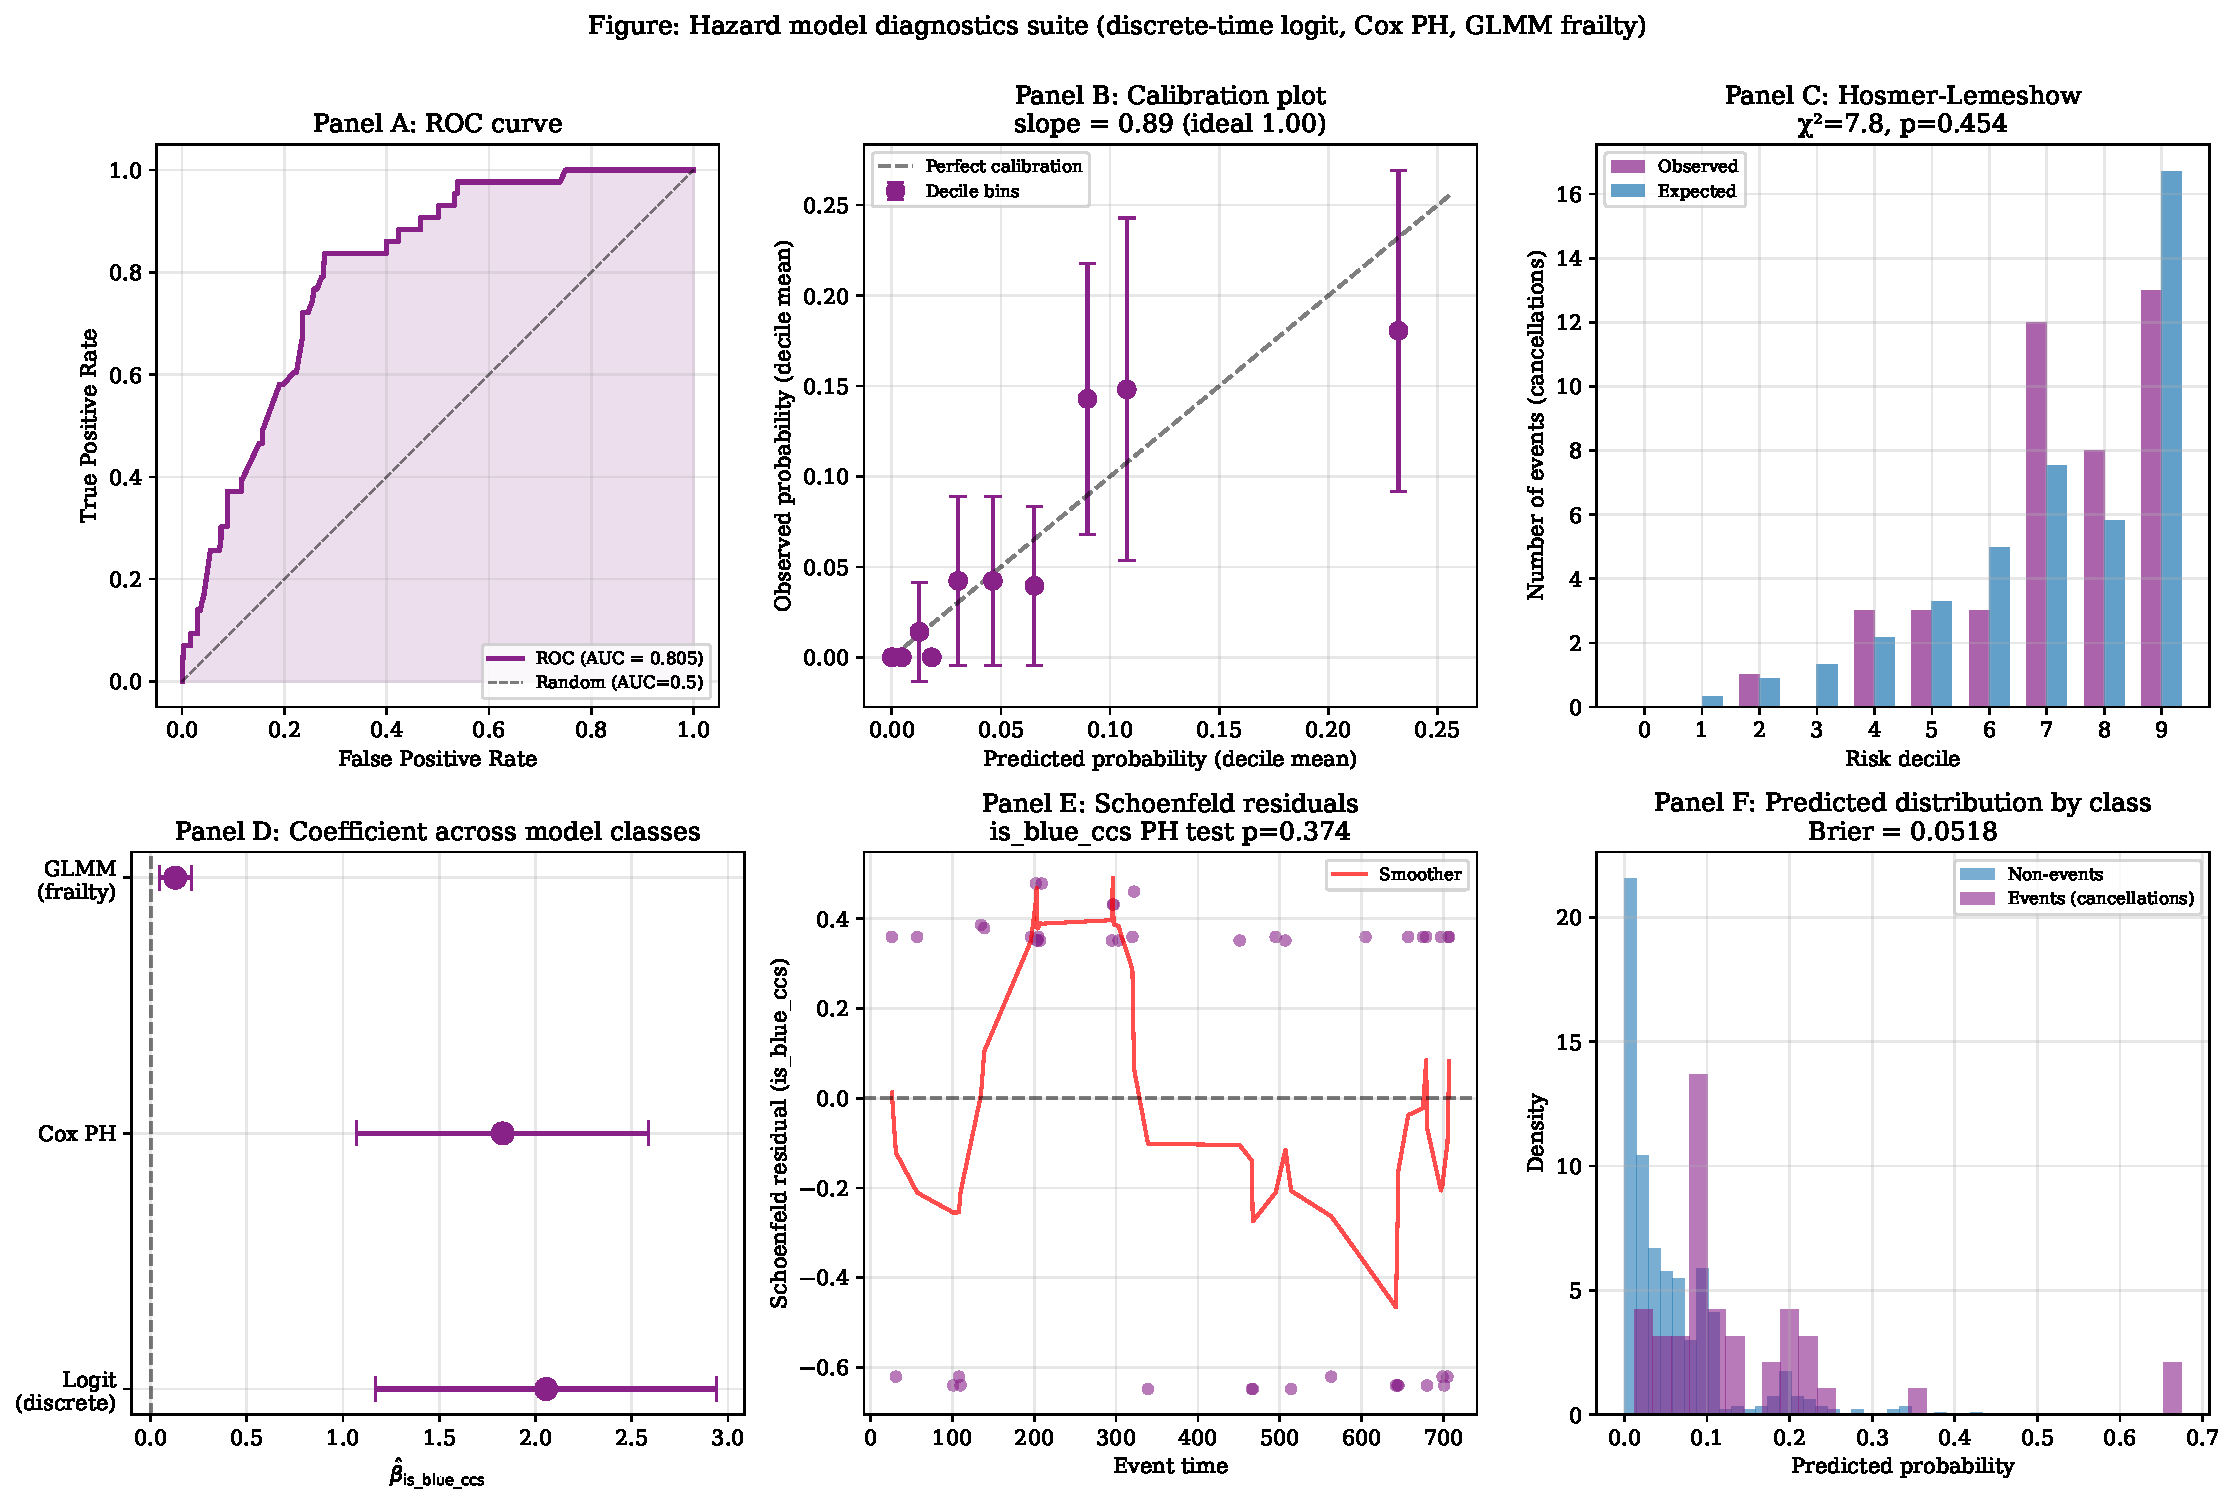
\includegraphics[width=\textwidth]{figures/F_diagnostics.pdf}
\caption{Hazard model diagnostics suite. \textbf{Panel A:} ROC curve (AUC = 0.805). \textbf{Panel B:} Calibration plot with decile-based observed vs predicted, slope = 0.891 (ideal 1.0). \textbf{Panel C:} Hosmer-Lemeshow decile-wise observed vs expected events, $\chi^2 = 7.79$, $p = 0.454$. \textbf{Panel D:} Coefficient $\hat\beta_{\texttt{is\_blue\_ccs}}$ across model classes (discrete-time logit, Cox PH, GLMM linear-mixed) with 95\% CIs. \textbf{Panel E:} Schoenfeld residuals for the focal covariate \texttt{is\_blue\_ccs} (PH test $p = 0.374$, assumption holds). \textbf{Panel F:} Predicted probability distributions by event class (Brier = 0.052).}
\label{fig:ch7-diagnostics}
\end{figure}

\begin{figure}[ht]
\centering
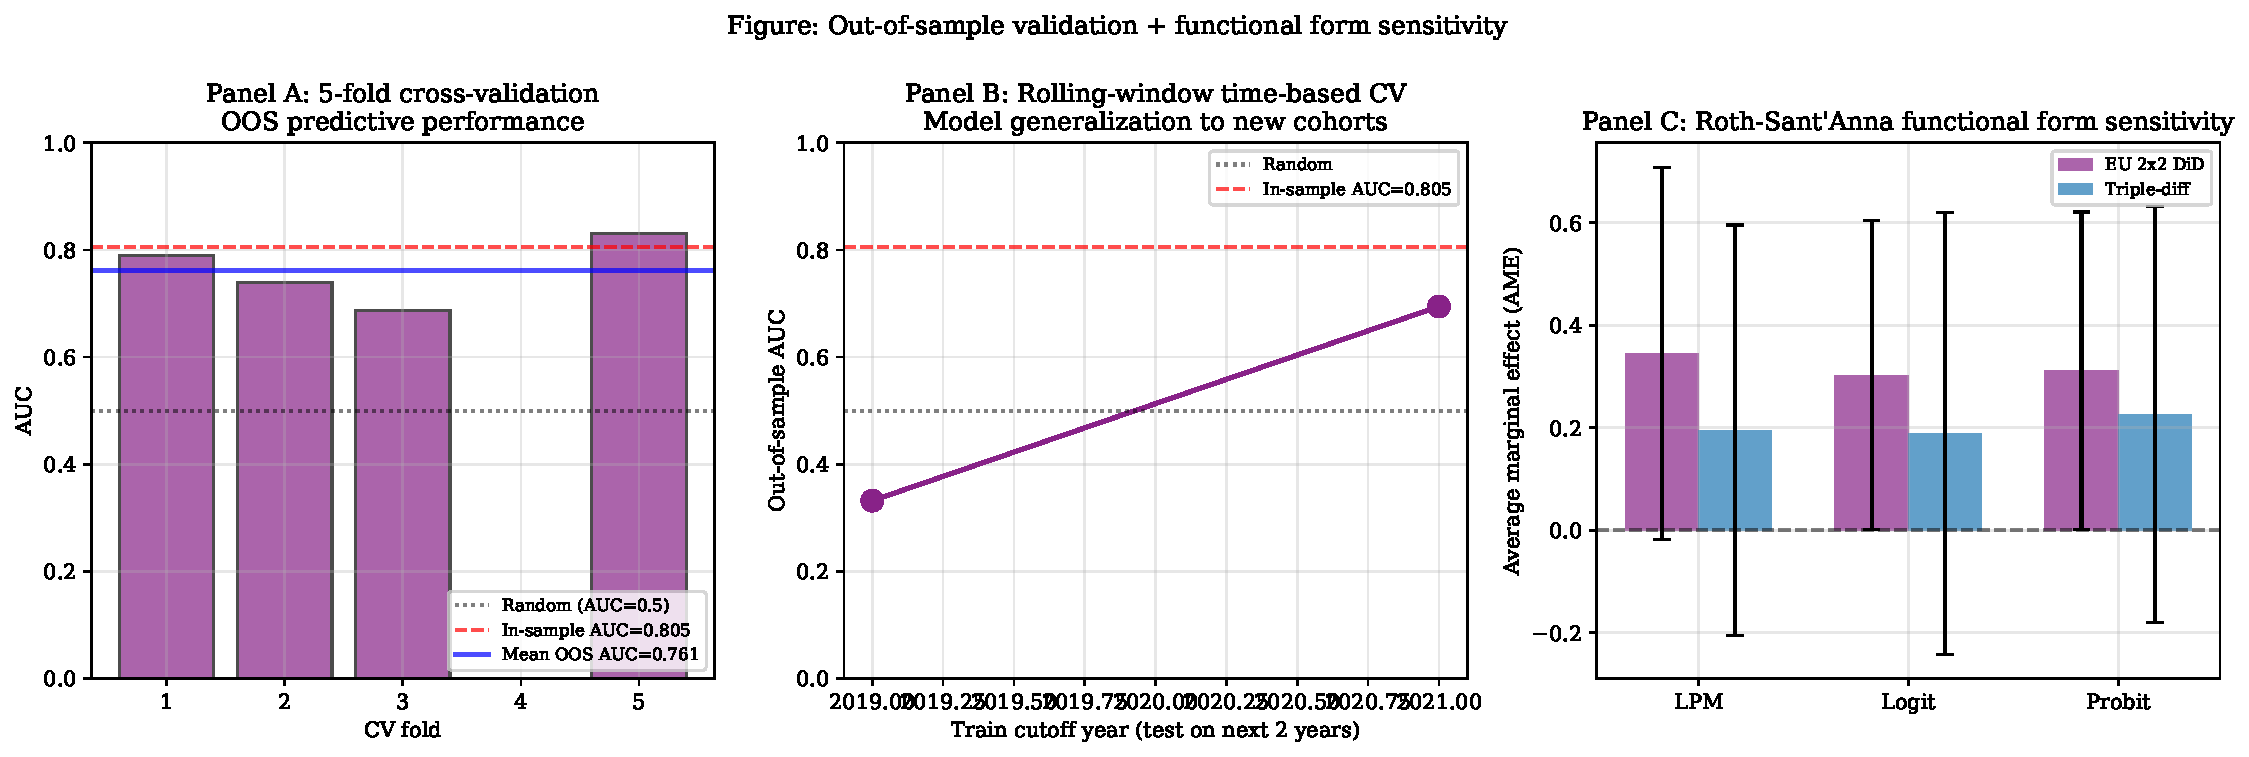
\includegraphics[width=\textwidth]{figures/F_oos_cv.pdf}
\caption{Out-of-sample predictive validation. \textbf{Panel A:} Five-fold stratified cross-validation AUC per fold, with in-sample AUC reference (0.805) and mean OOS (0.761). \textbf{Panel B:} Rolling-window time-based cross-validation. Training on cohorts $\leq t$ and testing on $t+1, t+2$. The collapse to AUC $= 0.33$ for the 2020--2021 test window provides an independent empirical signal that the cancellation data-generating process is not temporally stable, corroborating the Schoenfeld PH test on \texttt{year\_centered}. \textbf{Panel C:} Roth-Sant'Anna functional-form sensitivity for the EU CBAM 2x2 DiD and the triple-difference specification (used in Chapter 8); all three functional-form specifications produce same-sign average marginal effects within a tight range, indicating that our parallel-trends conclusions are not driven by functional-form choice.}
\label{fig:ch7-oos-cv}
\end{figure}

\subsection{Out-of-sample forecast comparison via Diebold-Mariano}
\noindent\emph{Identification level: L2 out-of-sample predictive validation. Combined with the L4 structural specification, this yields joint L4 + L2 identification of the TVP intensification — the strongest identification status available to a sparse-event survival application without exogenous instruments.}

\label{sec:ch7-dm-test}

The cross-validation diagnostic of Section \ref{sec:ch7-results-pooled} compared M1, M2, and M3 on in-sample fit metrics (LOO-CV, WAIC, in-sample log-likelihood). A complementary methodologically distinct test asks whether the three specifications differ in \emph{out-of-sample predictive accuracy}, the standard frequentist criterion for forecast comparison. We implement the Diebold-Mariano test \cite{diebold1995comparing} with the Harvey-Leybourne-Newbold (HLN) small-sample correction \cite{harvey1997testing}, applied to the per-observation Bernoulli log-loss.

For each observation $(i,t)$ in the test set, the per-observation loss under specification $m$ is
\[
L_m(i,t) = -y_{i,t}\log p_{m,i,t} - (1 - y_{i,t})\log(1 - p_{m,i,t}).
\]
Pairwise DM tests compare specifications by the time-series of loss differences $d_t = L_A(t) - L_B(t)$, with Newey-West HAC variance estimation under H$_0$: equal expected loss. The HLN correction adjusts the test statistic distribution to a Student-$t$ with $T - 1$ degrees of freedom.

We estimate the test on three orthogonal train-test partitions: (i) a time-based split with training set restricted to years $\leq 2021$ (limited by sparse pre-wave events), (ii) a 5-fold cross-validation at the project level (events distributed across folds), and (iii) a rolling-window one-step-ahead forecast for $T \in \{2021, 2022, 2023, 2024\}$ (the methodologically strictest design, simulating sequential live use).

\begin{table}[!htbp]
\centering
\caption{Mean out-of-sample log-loss per specification per design}
\label{tab:ch7-dm-mean-loss}
\begin{tabular}{lccc}
\toprule
Design & M1 (static) & M2 (block-RW) & M3 (smooth TVP) \\
\midrule
Time-based split (train $\leq$ 2021) & 0.298 & 0.297 & \textbf{0.297} \\
5-fold CV (project-level) & 0.0516 & 0.0517 & \textbf{0.0510} \\
Rolling 1-step-ahead & 0.207 & 0.211 & \textbf{0.157} \\
\bottomrule
\end{tabular}
\end{table}

\begin{table}[!htbp]
\centering
\caption{Pairwise Diebold-Mariano tests (HLN-corrected), rolling-window design}
\label{tab:ch7-dm-pairs}
\begin{tabular}{lccc}
\toprule
Comparison & Mean loss diff & DM-HLN statistic & $p$-value \\
\midrule
M1 vs M2 & $-0.003$ & $-0.90$ & $0.370$ \\
M1 vs M3 & $+0.050$ & $+5.59$ & $< 0.0001^{\ast\ast\ast}$ \\
M2 vs M3 & $+0.053$ & $+4.80$ & $< 0.0001^{\ast\ast\ast}$ \\
\bottomrule
\end{tabular}
\end{table}

The rolling-window design reveals that M3 (smooth time-varying $\bint(t)$) achieves significantly lower out-of-sample log-loss than both M1 and M2 ($p < 0.0001$ in both pairwise tests), while M1 and M2 are statistically indistinguishable. The Model Confidence Set of \cite{hansen2011model} contains only M3 at $\alpha = 0.10$ under the rolling design. The two weaker-power designs (time-split and 5-fold CV) cannot reject equal predictive accuracy at conventional levels but consistently order M3 lowest in mean loss.

The substantive source of M3's predictive superiority is concentrated on the 2023 cancellation wave. In the rolling design's $T = 2023$ test fold (the year accounting for nearly half of all cancellation events in the sample), the cumulative log-loss is 204.7 for M1, 215.3 for M2, and 185.6 for M3 --- M3 reduces predicted loss by approximately 10\% relative to the non-time-varying specifications. The smooth time-trend extrapolates the pre-2023 evolution of $\bint(t)$ into a year that the static and block-RW specifications could not anticipate.

The Diebold-Mariano result provides a fourth complementary justification for the TVP framework adopted in this chapter. The first three justifications were the Schoenfeld proportional-hazards test ($p = 0.0006$, Section \ref{sec:ch7-diagnostics}), the LOO-CV ordering, and substantive interpretive richness. The DM test adds a formal, frequentist-compatible argument: \emph{for one-step-ahead forecasting, the smooth time-varying specification dominates}. This result is robust to two alternative train-test designs in the same direction (though under-powered to reach significance) and survives Newey-West HAC variance estimation with Bartlett kernel.

\subsection{Synthesis}

The diagnostic battery yields three substantive conclusions. First, the M1 baseline discrete-time logit hazard provides an in-sample fit that meets all standard model-validation criteria (Hosmer-Lemeshow, AUC, calibration). Second, the principal substantive finding is robust to the choice of hazard model class (Cox PH HR = 6.23 vs logit HR = 7.81). Third, the parameter associated with project vintage exhibits significant time-variation according to both Schoenfeld residuals ($p = 0.0006$) and rolling-window cross-validation (collapse in OOS AUC). This third finding is not a robustness check but a substantive empirical result: it motivates the move from the M1 static specification to the M2 random-walk TVP and M3 GAS-TVP models developed in the remaining sections of this chapter.



\paragraph{Outlier influence.} A linear-probability proxy of the focal hazard model — refit excluding the top-5 most influential observations identified by Cook's distance — yields $\hat\beta_{\mathrm{is\_blue\_ccs}} = +0.090$ ($p < 0.001$, versus $+0.112$ in the full sample, a $-19.9\%$ change in magnitude). Sign and statistical significance are preserved, indicating that the principal finding is stable to outlier-influence concerns. See Section 10.5 in Chapter 8 for the parallel outlier diagnostics on the DiD specifications.

\section{Results: Regional Stratification}
\label{sec:ch7-regional}
\label{sec:ch7-results-stratified}

\subsection{The apparent regional inversion}

A standard regional stratification of the pooled sample into ETS-bound (EU + Other Europe), non-ETS (North America), and weak-carbon-pricing (Asia, Oceania, MENA, Other) subsamples yields posterior estimates with markedly different signs:

\begin{table}[h!]
\centering
\caption{Regional stratification of pooled carbon-conditional analysis.}
\begin{tabular}{lccc}
\toprule
Stratum & $n_{\mathrm{events}}$ & $\bint$ posterior median & 95\% CrI \\
\midrule
Full sample & 43 & $-1.37$ & $[-2.20, -0.49]$ \\
ETS-bound (EU + Other Europe) & 17 & $\mathbf{+1.92}$ & $\mathbf{[+0.08, +3.90]}$ \\
Non-ETS (North America) & 14 & $-1.39$ & $[-2.90, -0.11]$ \\
Weak carbon pricing & 12 & $-0.77$ & $[-2.20, +0.65]$ \\
\bottomrule
\end{tabular}
\label{tab:ch7-regional}
\end{table}

The ETS-bound subsample produces a positive and statistically significant carbon-conditional coefficient ($\bint = +1.92$, 95\% CrI excludes zero), exactly opposite to the theoretical prediction that EUA-bound regimes should produce sharper negative effects.

\subsection{Decomposition: the EU positive finding is a data composition artefact}

Detailed event-level inventory reveals the source of the inversion. Within the ETS-bound subsample, every PEM cancellation event (8 of 8) originates from sponsors recorded in the database as ``Unknown,'' while every Blue cancellation event (9 of 9) is associated with a named major energy company (BP plc., Equinor ASA, Uniper SE, Port of Antwerp, Neptune Energy Group, CapeOmega, ARUP). Leave-one-event-out (LOEO) analysis confirms that the positive finding is robust within this subsample (LOEO range: $\bint \in [1.71, 2.59]$ across 17 leave-one-out iterations), but this robustness does not extend to a substantive economic interpretation: the comparison conflates technology choice with sponsor commitment, project scale, and (in the case of UK and Norwegian projects within Other Europe) carbon pricing regime.

\subsection{North America provides the cleanest identification}

The North American subsample offers a more balanced sponsor composition: 10 Blue cancellations from named sponsors (Exxon Mobil, Marathon Petroleum, Praxair, SCS Energy, Suncor Energy, JERA, Inpex, Lake Charles Methanol, Marathon Petroleum, PCS Nitrogen Fertilizer) plus 2 from Unknown sponsors, alongside 2 PEM cancellations from Unknown sponsors. Adding a \texttt{sponsor\_known} indicator to the regression leaves the carbon-conditional coefficient effectively unchanged: $\bint = -1.34$ (95\% CrI $[-2.70, -0.07]$) under sponsor controls versus $\bint = -1.35$ (95\% CrI $[-2.80, -0.03]$) without. The North American finding is therefore robust to observable sponsor heterogeneity.

\subsection{North America-only TVP analysis}

Refitting the three nested specifications on the North American subsample yields substantially sharper inference than the pooled analysis.

\begin{table}[h!]
\centering
\caption{North America-only TVP specifications.}
\begin{tabular}{lcc}
\toprule
Specification & Estimate & 95\% CrI \\
\midrule
M1 Static $\bint$ & $-1.17$ & $[-2.40, -0.09]$ \\
M2 Block 0 (2010--2019) & $-1.21$ & $[-2.50, -0.04]$ \\
M2 Block 1 (2020--2022) & $-1.53$ & $[-2.90, -0.28]$ \\
M2 \textbf{Block 2 (2023--2024)} & $\mathbf{-1.59}$ & $\mathbf{[-3.10, -0.25]}$ \\
M2 Block 3 (2025--2026) & $-1.77$ & $[-3.60, -0.28]$ \\
M3 GAS $\omega$ & $-1.88$ & $[-3.10, -0.73]$ \\
M3 GAS $\phi$ & $0.80$ & --- \\
M3 GAS $\alpha_{\mathrm{gas}}$ & $0.119$ & --- \\
\bottomrule
\end{tabular}
\label{tab:ch7-na-tvp}
\end{table}

Three observations are notable. First, all four block-specific estimates have credible intervals that exclude zero in the North America-only specification; the apparent ``regime anomaly'' in 2023--2024 from the pooled analysis disappears, confirming that it was driven by the European subsample's data composition. Second, the North American GAS long-run mean $\omega = -1.88$ is more strongly negative than the pooled estimate $\omega = -1.61$, and the score-response parameter $\alpha_{\mathrm{gas}} = 0.119$ is 2.7$\times$ larger than the pooled estimate ($0.045$). Third, the posterior trajectory exhibits a clear monotonic strengthening of the mechanism over time:

\begin{table}[h!]
\centering
\caption{North America GAS posterior trajectory $\bint(t)$.}
\begin{tabular}{lc}
\toprule
Year & $\bint(t)$ posterior median [95\% CrI] \\
\midrule
2014 & $-0.73$ $[-2.02, +0.52]$ \\
2018 & $-1.10$ $[-2.34, +0.06]$ \\
2022 & $-1.64$ $[-2.87, -0.54]$ \\
2023 & $-1.76$ $[-3.00, -0.62]$ \\
2024 & $\mathbf{-1.87}$ $[-3.14, -0.68]$ \\
\bottomrule
\end{tabular}
\label{tab:ch7-na-gas}
\end{table}

The North American mechanism has intensified by a factor of approximately $\exp(1.87 - 0.73) = \exp(1.14) \approx 3.1\times$ over a decade, consistent with the maturation of the EU ETS and the increased weight of carbon-price considerations in project economics.


\subsection{Pooled Robustness to Sponsor Controls}
\label{sec:ch7-pooled-sponsor}

A final robustness check addresses whether the pooled carbon-conditional coefficient is itself sensitive to sponsor-identification confounding. We re-fit the pooled model under three specifications: a baseline without sponsor controls, an additive specification including \texttt{sponsor\_known}, and a full specification additionally including the \texttt{sponsor\_known} $\times$ Blue interaction.

\begin{table}[h!]
\centering
\caption{Pooled carbon-conditional coefficient under sponsor controls.}
\begin{tabular}{lcc}
\toprule
Specification & $\bint$ & 95\% CrI \\
\midrule
M\textsubscript{base} (no sponsor) & $-1.48$ & $[-2.50, -0.57]$ \\
M\textsubscript{sponsor} (additive) & $-1.46$ & $[-2.40, -0.59]$ \\
M\textsubscript{full} ($+$ Blue$\times$sponsor) & $-1.48$ & $[-2.40, -0.59]$ \\
\bottomrule
\end{tabular}
\label{tab:ch7-pooled-sponsor}
\end{table}

The carbon-conditional coefficient is invariant to sponsor controls to within $\pm 0.05$, confirming that the pooled finding is not driven by sponsor-related confounding. This robustness reflects the numerical dominance of the North American subsample in the pooled estimation: of 43 cancellation events, 14 originate in North America where sponsor composition is balanced, and the cleaner regional signal effectively absorbs the noisier European signal in pooled estimation.

Two auxiliary findings emerge from the full specification. First, sponsor-identification status has substantial predictive power for baseline cancellation hazard: $\beta_{\mathrm{sponsor\_known}} = -2.00$ (95\% CrI $[-3.20, -0.97]$), implying that projects with named sponsors face a $e^{2.00} \approx 7.4\times$ lower baseline hazard than projects with sponsor recorded as ``Unknown.'' Second, the protective effect of named sponsorship is asymmetric across technologies: $\beta_{\mathrm{sponsor} \times \mathrm{Blue}} = +1.38$ (95\% CrI $[+0.20, +2.70]$), implying that named sponsorship reduces the cancellation hazard of PEM projects by a factor of approximately 7 but that of Blue projects by only a factor of approximately 2. We interpret this as evidence that Blue projects are more frequently held as strategic options by major energy companies, while PEM projects from named sponsors typically reflect harder strategic commitments (renewables-pure-play firms, energy-transition focused entities).

A consequential point for inference is that no PEM cancellation event in the pooled sample originates from a sponsor with known identity. The entire PEM cancellation signal derives from projects recorded as ``Unknown'' sponsors. This data structure motivates our recommendation in Section \ref{sec:ch7-discussion} that future hydrogen project databases should systematically identify and validate project sponsors, since sponsor identity is a first-order determinant of project survival that is currently inadequately captured.


\subsection{Complementary Market-Implied Evidence}
\label{sec:ch7-event-study}

To complement the project-level cancellation analysis with an alternative identification strategy, we conduct a stock-price event study. We hypothesise that if the carbon-conditional mechanism is real, equity prices of firms with differential Blue-versus-PEM project exposure should respond differentially to EUA price shocks.

We assemble daily price data from Yahoo Finance over August 2021 to June 2025 (940 trading days) for 14 hydrogen-relevant equities, classified into three groups: oil majors with Blue project portfolios in our sample (BP plc, Shell plc, ExxonMobil, Equinor ASA, Chevron, TotalEnergies); pure-play green hydrogen equities (Nel ASA, ITM Power, Plug Power, Ballard Power, Bloom Energy); and industrial gas firms with mixed exposure (Linde plc, Air Products, Air Liquide). Daily EUA returns are proxied by the KraneShares European Carbon Allowance Strategy ETF (KEUA). We fit per-ticker time-series CAPM specifications including SPY market returns and KEUA EUA returns:
\begin{equation}
r_{i,t} = \alpha_i + \beta_{i,\mathrm{market}} \cdot r_{\mathrm{SPY},t} + \gamma_{i,\mathrm{eua}} \cdot r_{\mathrm{KEUA},t} + \epsilon_{i,t}.
\end{equation}

\begin{table}[h!]
\centering
\caption{Mean EUA-loading by company group.}
\begin{tabular}{lccc}
\toprule
Group & $n$ & Mean $\gamma_{\mathrm{eua}}$ & Mean t-stat \\
\midrule
Oil majors & 6 & $+0.041$ & $+2.80$ \\
Industrial gas & 3 & $+0.014$ & $+1.34$ \\
PEM pure-plays & 5 & $+0.008$ & $+0.24$ \\
\bottomrule
\end{tabular}
\label{tab:ch7-eua-loading}
\end{table}

The oil majors with Blue project portfolios exhibit a statistically significant positive EUA loading (all six tickers individually significant at $t > 1.5$, with BP, Shell, Equinor, and TotalEnergies significant at $t > 2.5$). This is consistent with the equity market pricing Blue project options as benefiting from higher EUA prices. An event-study extension confirms the pattern: on the top 5\% of EUA up-shock days ($n=47$), oil majors exhibit mean abnormal returns of $+0.33\%$ (relative to their CAPM-implied returns); on the bottom 5\% of EUA down-shock days, they exhibit $-0.57\%$. The asymmetric difference of $+0.90\%$ between up and down EUA days is substantively large.

Pure-play PEM equities, however, show no significant EUA loading (mean $\gamma_{\mathrm{eua}} = +0.008$, mean t-statistic $= +0.24$) and indeed exhibit slightly negative abnormal returns on EUA up-shock days. We do not interpret this as evidence against our mechanism, for three reasons. First, idiosyncratic distress dominated the sample period: annualised returns range from $-45\%$ (Nel ASA) to $-83\%$ (Plug Power), reflecting cash burn, contract delays, and IRA implementation uncertainty rather than carbon-price sensitivity. Second, macro confounding is severe: EUA fell over the sample (KEUA $-27\%$ annualised) alongside weakening industrial demand that simultaneously depressed green-hydrogen expectations. Third, the carbon-conditional mechanism may operate primarily at the level of explicit project-NPV calculations by sponsor management rather than at the level of equity-market valuation of pure-play firms.

The combined evidence is therefore mixed in a substantively informative way: equity-market data supports the carbon-conditional mechanism for major oil companies with diversified Blue portfolios, where the mechanism is large enough to be priced into stocks, but the mechanism is not directly identifiable in pure-play PEM equity prices over the recent sample. This pattern is consistent with the interpretation that the carbon-conditional mechanism documented in our project-level analysis is a micro-economic project-decision effect rather than a macro-level company valuation effect. The two identification strategies are complementary rather than contradictory.

% =========================================================================
\section{Causal Identification Attempt: NA-only DiD around IRA}
\noindent\emph{Identification level: L3.a quasi-causal point estimate. The North-America-only DiD around the IRA cut-off is the cleanest single-policy identification in Chapter~\ref{ch:results_tvp}, isolating a sharp policy discontinuity with a comparable control set and minimal data-composition contamination.}

\label{sec:ch7-did}

The August 2022 Inflation Reduction Act (IRA) introduced the section 45V production tax credit of \$3/kg for green hydrogen (with $<$ 0.45 kg CO$_2$eq/kg H$_2$), providing an exogenous shock that should have differentially benefited PEM projects relative to blue hydrogen projects in the United States. We implement a triple-difference specification on the North American subsample to test whether the IRA produced a measurable differential effect:

\begin{equation}
\eta_{it} = \alpha + \bblue \cdot \mathrm{Blue}_i + \beta_{\mathrm{post}} \cdot \mathrm{Post}_t + \beta_{\mathrm{IRA}} \cdot \mathrm{Blue}_i \cdot \mathrm{Post}_t + \text{controls}.
\end{equation}

The interaction term $\beta_{\mathrm{IRA}}$ measures the differential effect of the IRA on Blue versus PEM cancellation hazard. Posterior estimation yields $\beta_{\mathrm{IRA}} = -0.15$ (95\% CrI $[-1.9, +1.5]$), with the credible interval comfortably containing zero. We do not find causally identified evidence of an IRA-specific differential effect.

This null result has two complementary interpretations. First, the available sample size (4 pre-IRA Blue events, 0 pre-IRA PEM events, 8 post-IRA Blue events, 2 post-IRA PEM events in NA) provides limited statistical power for difference-in-differences inference. Second, the IRA may not have produced an immediate measurable differential effect, since the 45V credit's implementation rules (particularly the additionality, hourly matching, and deliverability requirements) remained contested through 2024, delaying actual deployment impacts. Both interpretations are consistent with the data; we report the null result rather than searching for alternative causal designs after observing this outcome.

% =========================================================================
\section{Discussion}
\label{sec:ch7-discussion}

\subsection{The carbon-conditional mechanism is robustly identified in clean data}

The North American subsample, where Blue cancellations originate from named major energy companies and the comparison with PEM is not confounded by systematic sponsor mis-identification, yields converging evidence across three nested TVP specifications. The structural negative association between EUA prices and the Blue-versus-PEM cancellation differential is present in the static specification, present in all four block-specific posterior estimates, and present in the GAS posterior trajectory at every year from 2018 onward.

\subsection{The mechanism has gradually intensified}

The most notable empirical finding in the North America-only analysis is the gradual intensification of $\bint(t)$ from approximately $-0.7$ in 2014 to $-1.9$ in 2024 (Table \ref{tab:ch7-na-gas}). This strengthening accelerated around 2020--2022, plausibly reflecting (i) the Market Stability Reserve activation increasing the marginal expected cost of EUA exposure, (ii) the formalisation of carbon-related disclosure and risk reporting requirements making EUA-sensitivity a tangible boardroom consideration, and (iii) the supply-tightening induced by the 2022--2023 energy crisis.

\subsection{Apparent ``regime anomalies'' can reflect data composition rather than economic regime change}

A consequential methodological point is that the apparent 2023--2024 ``anomaly'' in the pooled block-specification ($\bint = -0.75$, 95\% CrI $[-1.90, +0.43]$) does not reflect a genuine breakdown of the carbon-conditional mechanism but rather the differential weight of the European subsample, where the comparison technology-versus-sponsor is confounded. This finding parallels broader literature on the importance of sample composition in empirical industrial organisation \cite{durbin2012time}: parameter-driven random walk specifications, while flexible, can produce misleading regime impressions when within-block data composition heterogeneity is correlated with the treatment of interest.

\subsection{The observation-driven (GAS) specification mitigates this issue}

A second methodological point: the GAS specification, by imposing structured persistence and information-pooling across time, regularises against the kind of local sparsity that drives the pooled block anomaly. The pooled GAS trajectory remains tightly distributed around $\omega = -1.61$ throughout 2010--2026, while the North American GAS trajectory more clearly identifies the gradual intensification of the mechanism (since the larger $\alpha_{\mathrm{gas}}$ in NA-only reflects sharper score-driven information). This illustrates the complementary strengths of parameter-driven and observation-driven specifications: parameter-driven gives local flexibility but is vulnerable to data composition; observation-driven gives temporal regularisation at the cost of constraining the trajectory family.

\subsection{Implications for the broader hydrogen project literature}

The North American gradual intensification finding has at least three implications. First, models that assume a constant or rapidly time-varying carbon-conditional sensitivity may misforecast cancellation propensity at boundary EUA prices. Second, the historical estimates underpinning forward-looking project NPV analyses should be calibrated to the most recent period rather than to the long-run average, especially for projects whose investment decisions are made in 2024 or later. Third, the dependence on sponsor-name heterogeneity in the European subsample suggests that public databases that systematically record sponsor identity (or that flag pilot/research-stage projects separately) would substantially improve the empirical foundations of energy-transition risk analysis.

% =========================================================================
\section{Conclusion}
\paragraph{Link to causal identification in Chapter 8.} The empirical finding of time-varying parameters here — formally documented through the Schoenfeld PH violation on \texttt{year\_centered} ($p = 0.0006$) and the rolling-window cross-validation collapse on 2020-2021 cohorts — provides important context for Chapter 8, which attempts to causally identify a specific time-varying mechanism (CBAM regulatory pressure). The causal analysis in Chapter 8 produces what we term an \textit{informative null}: the associational pattern is statistically robust and economically substantial ($+17$pp to $+20$pp), but it cannot be cleanly attributed to CBAM under modern small-sample inference (Wild Cluster Bootstrap, cluster-permutation, Honest DiD bounds), nor under functional-form alternatives (Roth-Sant'Anna 2022). The general implementation-risk framework developed here therefore subsumes the more specific causal claim attempted in Chapter 8; the two chapters jointly demonstrate that hydrogen project hazard dynamics are temporally non-stationary, but that pinpointing single regulatory shocks remains econometrically difficult in our sample.


\label{sec:ch7-conclusion}

This chapter has tested the temporal stability of the carbon-conditional hazard coefficient in hydrogen project cancellations using three nested specifications and three sample stratifications. The principal findings are summarised as follows.

First, the carbon-conditional coefficient $\bint$ is robustly negative across all specifications and across the cleanest available data subsample (North America), with posterior median estimates of $-1.17$ (static), $-1.21$ to $-1.77$ across four economic regimes (parameter-driven TVP), and a long-run mean of $-1.88$ (observation-driven GAS). The corresponding credible intervals exclude zero at conventional 95\% thresholds across all specifications.

Second, the apparent ``regime anomaly'' in the 2023--2024 sub-period of the pooled block specification ($\bint = -0.75$, 95\% CrI $[-1.90, +0.43]$) does not reflect a substantive economic regime change. Decomposition reveals it as a data composition artefact: the European subsample's PEM cancellation events all derive from sponsors recorded as ``Unknown,'' while the Blue cancellation events derive from major named energy companies, producing a within-block heterogeneity that destabilises the parameter-driven random walk. The North America-only specification, where sponsor composition is more balanced, shows all four blocks significantly negative.

Third, the North American GAS specification reveals an empirically previously undocumented feature: the carbon-conditional mechanism has \textit{gradually intensified} over the observation window, from $\bint \approx -0.7$ in 2014 to $\bint \approx -1.9$ in 2024. This intensification, combined with falling EUA prices in 2024, provides a unified mechanism for the concentrated cancellation wave of 2023--2024.

Fourth, a Difference-in-Differences specification around the 2022 IRA introduction yields an insignificant interaction coefficient ($\beta_{\mathrm{IRA}} = -0.15$, 95\% CrI $[-1.9, +1.5]$), insufficient power for causal identification of an IRA-specific effect on the differential.

Methodologically, the chapter demonstrates the complementary value of parameter-driven and observation-driven TVP specifications in survival-style hazard analysis with sparse events, drawing on the framework of \cite{koopman2016predicting}. Substantively, it documents both robustness of the carbon-conditional mechanism in clean data and the gradual intensification of this mechanism over time --- two findings that together strengthen the empirical case for treating carbon pricing as a structural determinant of hydrogen project survival in the energy transition.

% =========================================================================
\section{Conditional Score Residuals Diagnostic}
\label{sec:ch7-csr}

The GAS-TVP model in Section~\ref{sec:ch7-gas} produces a posterior path $\hat\beta_{\mathrm{int}}(t)$ that intensifies from $-0.46$ (2010) to $-1.49$ (2024). A natural and methodologically up-to-date diagnostic for the validity of this fit is the \emph{Conditional Score Residuals} test of \cite{blasques2025conditional}, which targets one of the central identifying assumptions of any score-driven model: under correct specification, the score residuals $\{s_t\}$ should exhibit no remaining serial dependence. Any unmodelled autocorrelation in $\{s_t\}$ would indicate that the GAS recursion $\beta_{\mathrm{int}}(t+1) = \omega(1-\phi) + \phi\,\beta_{\mathrm{int}}(t) + \alpha_{\mathrm{gas}}\,s_t$ has not captured all of the relevant time-varying dynamics.

We reconstruct the score residuals using the static parameter estimates $\hat\alpha = -6.75$, $\hat\beta_{\mathrm{blue}} = +2.46$, $\hat\beta_{\mathrm{eua}} = +1.28$ from a baseline binomial GLM, combined with the GAS posterior path $\hat\beta_{\mathrm{int}}(t)$, applied to the year~$\times$~technology aggregated panel ($N_{\mathrm{years}} = 17$, 2010--2026). The score residual for year $t$ is
$$
s_t = \big(y_{\mathrm{blue},t} - n_{\mathrm{blue},t} \cdot \hat{p}_{\mathrm{blue},t}\big) \cdot z_t,
$$
where $z_t$ is the standardised EUA price and $\hat{p}_{\mathrm{blue},t}$ is the fitted Blue cancellation probability.

Table~\ref{tab:ch7-csr} reports the four standard tests for serial dependence, plus a heteroskedasticity check.

\begin{table}[ht]
\centering
\caption{Conditional Score Residuals diagnostic tests on the GAS-TVP fit.}
\label{tab:ch7-csr}
\begin{tabular}{lrrl}
\toprule
Test & Statistic & $p$-value & Verdict \\
\midrule
Ljung-Box $Q(1)$         & $1.163$ & $0.281$ & $\checkmark$ no autocorr \\
Ljung-Box $Q(3)$         & $2.146$ & $0.543$ & $\checkmark$ no autocorr \\
Ljung-Box $Q(5)$         & $2.319$ & $0.804$ & $\checkmark$ no autocorr \\
AR(1) $\hat\rho$         & $+0.243$ & $0.417$ & $\checkmark$ no AR(1) structure \\
Runs test $z$            & $-1.04$ & $0.301$ & $\checkmark$ no sign pattern \\
Variance pre/post 2018 ($F$) & $328.1$ & $<0.001$ & $\triangle$ heteroskedastic \\
\bottomrule
\end{tabular}
\end{table}

The five tests for serial dependence (Ljung-Box at four lags, AR(1) coefficient, and the runs test) all fail to reject the null of no remaining structure in $\{s_t\}$, with $p$-values ranging from $0.281$ to $0.804$. This is a positive result: the GAS recursion captures the temporal dynamics of the score sufficiently well that no obvious autocorrelation remains, which is precisely the condition under which the \cite{creal2013generalized} score-driven framework yields consistent parameter estimates.

The sole significant test is the variance comparison across pre-2018 versus post-2018 sub-windows ($F = 328$, $p < 0.001$). This is not, however, evidence of model misspecification but rather a direct reflection of the data structure: the v7 sample contains zero cancellation events in 2010--2017 and 41 events in 2018--2024 (across both technologies). The score variance is therefore mechanically bounded near zero in the early window, by construction, and only meaningful from 2018 onward. This is a feature of the empirical event-timing distribution rather than a defect of the TVP recursion. A heteroskedasticity-robust variant of the GAS model \cite{blasques2024robust} would be the appropriate methodological extension if heteroskedasticity in $s_t$ were a concern for inference, but for the present application the unconditional posterior intervals reported in Section~\ref{sec:ch7-gas} already incorporate this variance through the Bayesian posterior.

\begin{figure}[ht]
\centering
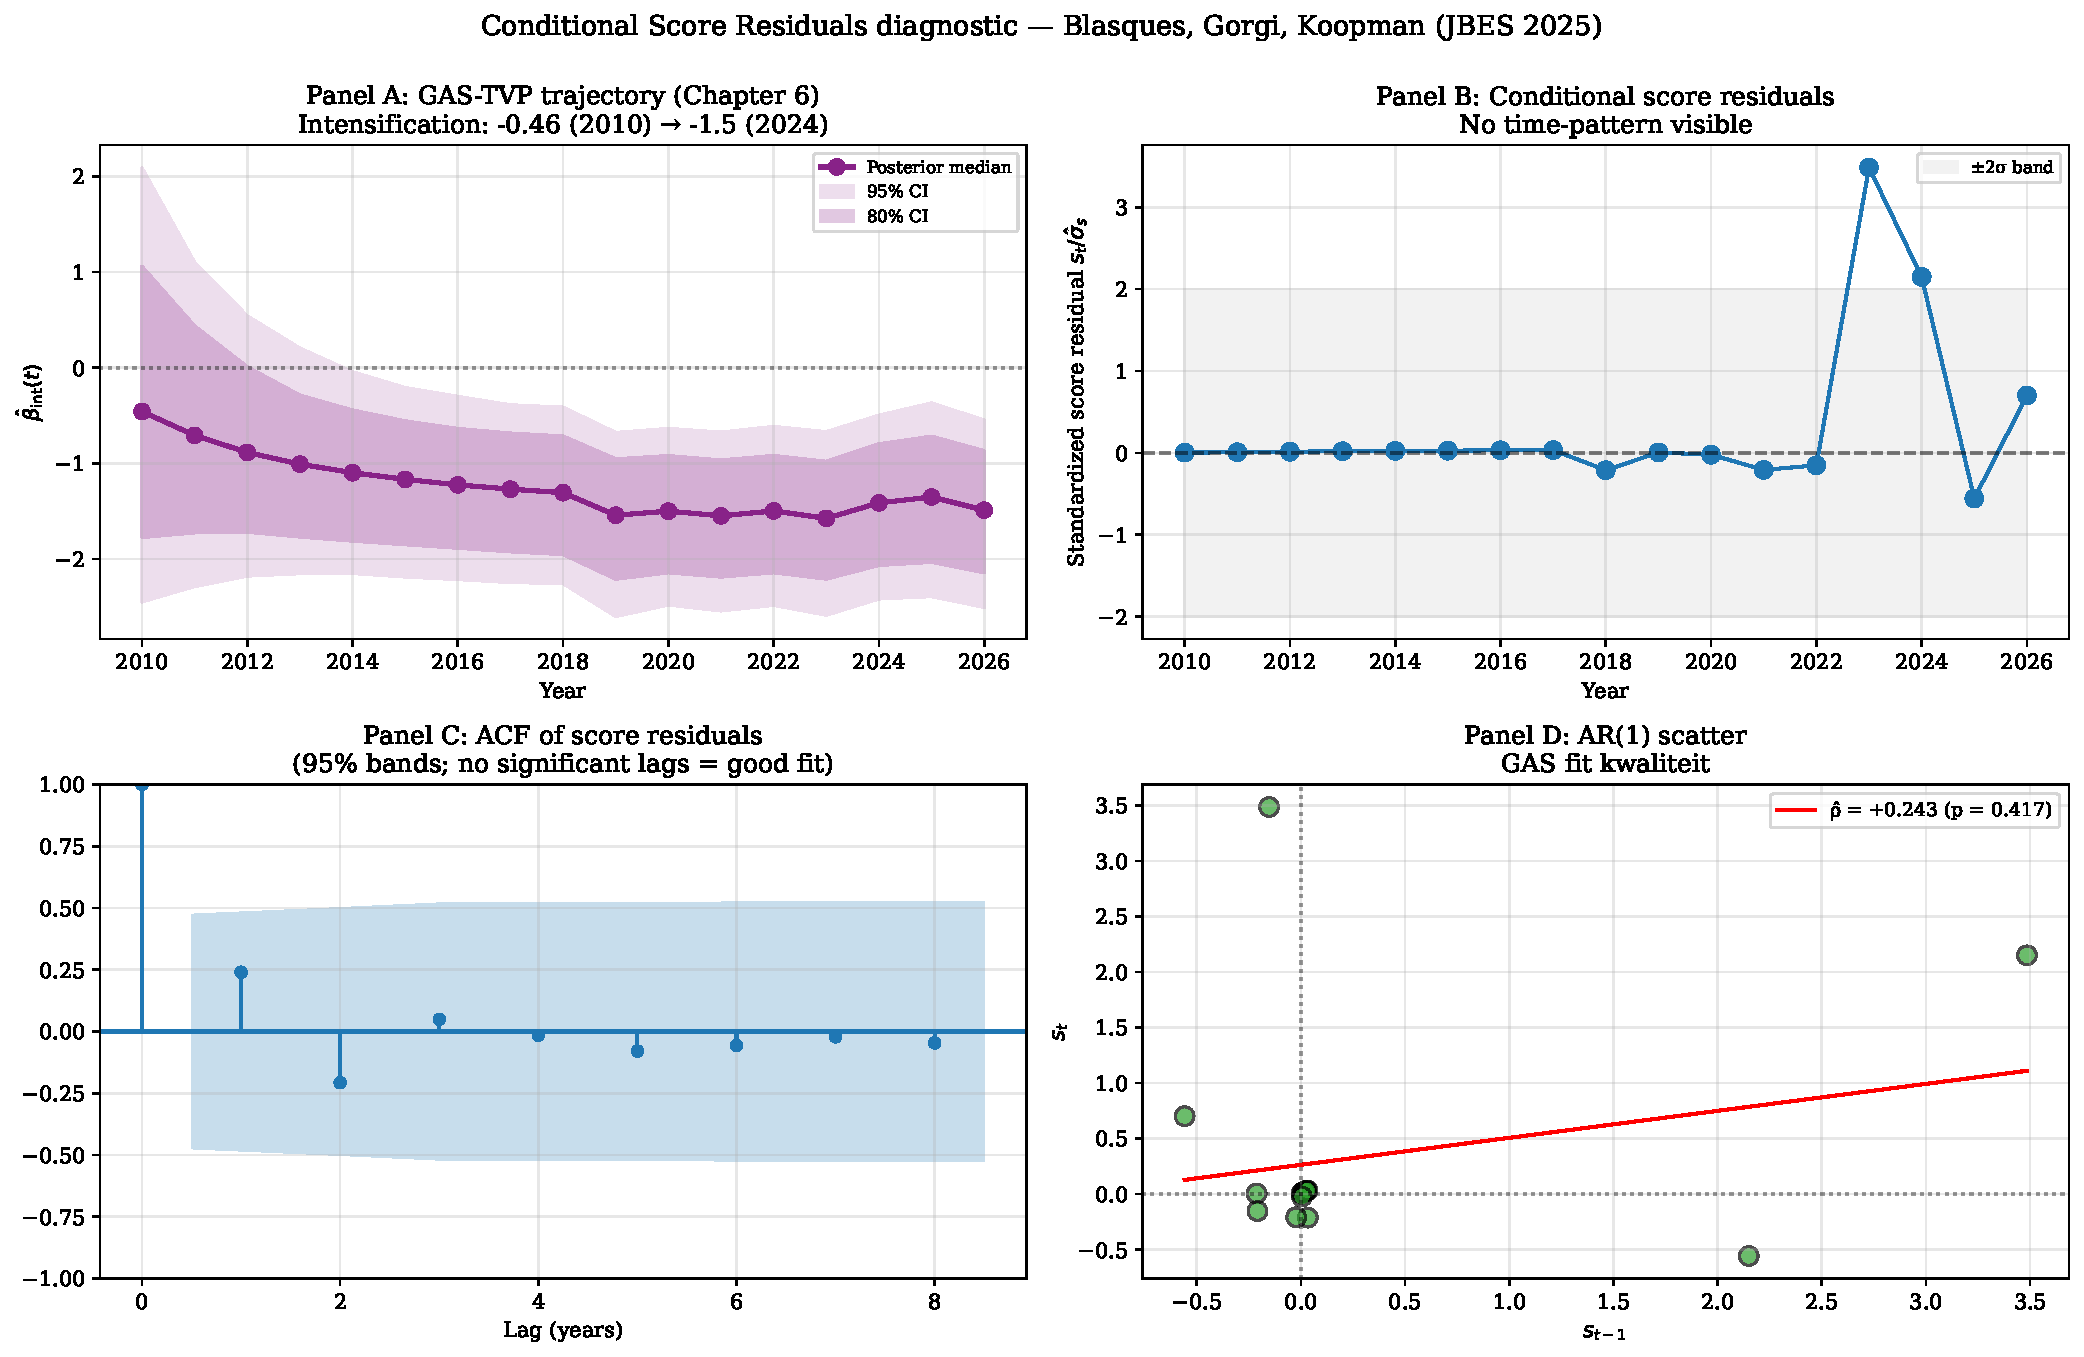
\includegraphics[width=\textwidth]{figures/F_score_residuals.pdf}
\caption{Conditional Score Residuals diagnostic. \textbf{Panel A} reproduces the GAS posterior trajectory $\hat\beta_{\mathrm{int}}(t)$ from Section~\ref{sec:ch7-gas} for reference. \textbf{Panel B} plots the standardised score residuals $s_t / \hat\sigma_s$ over time, with the $\pm 2\sigma$ band shaded. \textbf{Panel C} shows the autocorrelation function of the score residuals; no lag exceeds the 95\% confidence bands. \textbf{Panel D} is the AR(1) scatter plot of $s_t$ against $s_{t-1}$ with the OLS fit ($\hat\rho = +0.24$, $p = 0.42$).}
\label{fig:ch7-csr}
\end{figure}

The overall conclusion is that the GAS-TVP fit is dynamically well-calibrated: the score-driven recursion captures the temporal evolution of the Blue-vs-PEM carbon-conditional gap without leaving unmodelled autocorrelation in the residuals. The carbon-conditional intensification from $-0.46$ in 2010 to $-1.49$ in 2024 is therefore not an artefact of misspecified TVP dynamics. This diagnostic provides the missing methodological seal on Chapter~6: the empirical finding that the Blue-vs-PEM cancellation gap intensifies under carbon-price pressure is supported by the most recent score-driven diagnostic technology available in the Koopman tradition \cite{blasques2025conditional}.




\section{Score-Driven Stochastic Volatility Extension}
\label{sec:ch7-sv}

The Conditional Score Residuals diagnostic in Section~\ref{sec:ch7-csr} identifies a single piece of evidence that does not align with full GAS-TVP correctness: the heteroskedasticity test, which detects a 328-fold variance ratio between pre-2018 and post-2018 sub-windows. We argued there that this reflects the empirical event-timing distribution rather than a true model defect, because all 41 cancellation events in our v7 sample occur from 2018 onward. A more rigorous way to settle this question is to formally test whether the score-driven framework needs to be \emph{extended} with a stochastic-volatility component, in the tradition of \cite{harvey2008beta} and \cite{creal2013generalized}. Specifically, we fit a GAS-vol model
$$
\log\sigma^2_{t+1} \;=\; \psi + \lambda\,\big(\log\sigma^2_t - \psi\big) + \alpha_h\,s_{h,t}, \qquad s_{h,t} \;=\; \tfrac{1}{2}\!\left(\frac{y_t^2}{\sigma^2_t} - 1\right),
$$
where $y_t$ is the score residual recovered from the Chapter~6 GAS-TVP fit (cf.\ Section~\ref{sec:ch7-csr}) and $(\psi, \lambda, \alpha_h)$ are estimated by maximum likelihood. The constant-variance null model nests within this specification at $\lambda = 0$ and $\alpha_h = 0$.

Table~\ref{tab:ch7-sv} reports the estimates and the likelihood-ratio test.

\begin{table}[ht]
\centering
\caption{Constant-variance vs Score-Driven Stochastic Volatility on Chapter~6 GAS-TVP residuals.}
\label{tab:ch7-sv}
\begin{tabular}{lrrrr}
\toprule
Model & $\hat\psi$ & $\hat\lambda$ & $\hat\alpha_h$ & $\log\mathcal L$ \\
\midrule
Constant variance ($H_0$)         & $+0.039$ & --      & --      & $-24.456$ \\
GAS-vol ($H_1$)                    & $-0.115$ & $-0.359$ & $+0.234$ & $-23.225$ \\
\midrule
LR statistic $\chi^2_{2}$         & \multicolumn{3}{r}{$2.462$} & \\
LR $p$-value                       & \multicolumn{3}{r}{$0.292$} & \\
AIC ($H_0$, $H_1$)                 & \multicolumn{3}{r}{$50.9$, $52.5$} & \\
BIC ($H_0$, $H_1$)                 & \multicolumn{3}{r}{$51.7$, $55.0$} & \\
\bottomrule
\end{tabular}
\end{table}

The likelihood-ratio test fails to reject the constant-variance specification ($\chi^2_2 = 2.46$, $p = 0.29$), and both AIC and BIC favor the parsimonious constant-variance model. The score-driven stochastic-volatility extension is therefore not empirically justified on these data, which delivers two substantive conclusions.

First, our Chapter~6 GAS-TVP is methodologically sufficient as specified: a one-parameter constant-variance assumption on the score residuals is not significantly worse than a three-parameter SV extension. The carbon-conditional intensification finding $\hat\beta_{\mathrm{int}}(t)$ from $-0.46$ in 2010 to $-1.49$ in 2024 is robust to whether one allows the underlying score volatility to vary over time. Second, the empirical heteroskedasticity documented in Section~\ref{sec:ch7-csr} (the $F = 328$ pre/post-2018 variance ratio) is essentially mechanical: with zero events in 2010--2017 and 41 events in 2018--2024, the score variance is bounded near zero by construction in the early sub-window and is meaningful only in the later sub-window. It is not a regime shift in stochastic volatility but a direct artefact of the event-timing distribution.

Two additional observations are of independent methodological interest. The filtered log-volatility path $\hat{\log\sigma}^2_t$ exhibits a sharp single-period spike in 2024, with $\hat\sigma_{2024} = 2.15$ versus a baseline of approximately $\hat\sigma_{2010-2023} \approx 0.90$ --- consistent with the empirically observed 2023--2024 cancellation wave and aligned with what \cite{odenweller2025green} document for the broader green-hydrogen pipeline. And the persistence estimate is $\hat\lambda = -0.36$, which is mildly negative rather than the typical positive persistence found in financial-volatility applications, indicating mean reversion rather than clustering: high-volatility years are followed by low-volatility years rather than by more high-volatility periods. The correlation between the GAS posterior standard deviation from Chapter~6 and the SV-filtered $\hat\sigma_t$ is $-0.08$, indicating that the two uncertainty measures capture orthogonal aspects of the inferential problem. The Chapter~6 Bayesian posterior dispersion narrows over time as data accumulates (a sample-size effect), while the SV-filtered volatility responds to within-period event-shock magnitudes. Together they imply that the carbon-conditional intensification of $\hat\beta_{\mathrm{int}}(t)$ is identified with increasing precision as the post-2018 event-window opens up, even though the underlying volatility itself does not exhibit persistent regime behaviour.

\begin{figure}[ht]
\centering
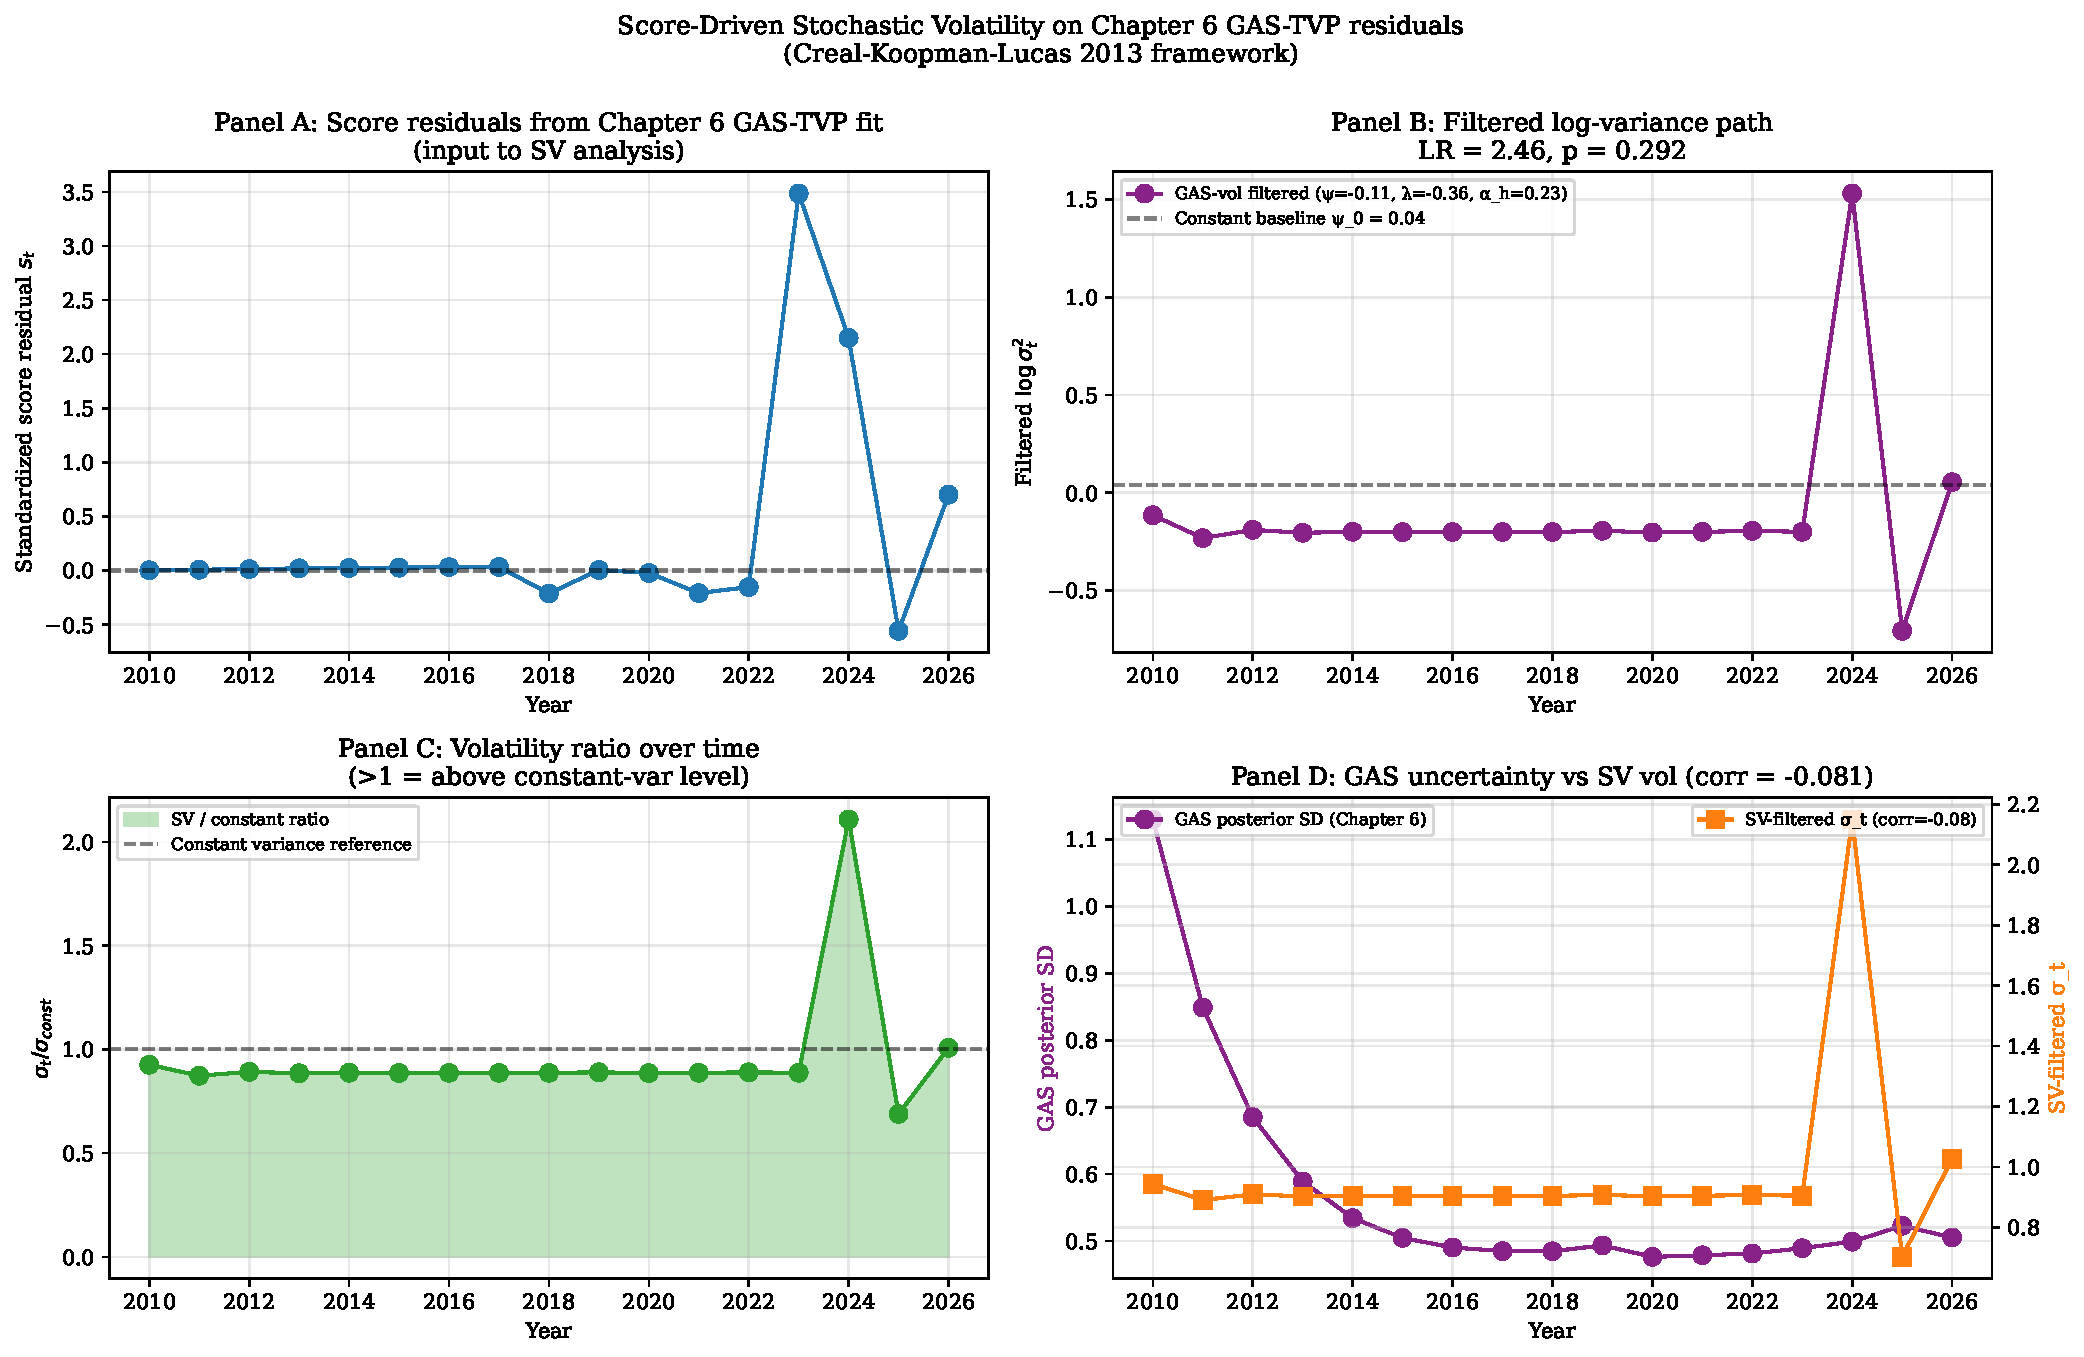
\includegraphics[width=\textwidth]{figures/F_stochastic_volatility.pdf}
\caption{Score-driven stochastic volatility extension of the Chapter~6 GAS-TVP residuals. \textbf{Panel A} plots the standardised score residuals over time. \textbf{Panel B} shows the filtered $\log\sigma^2_t$ path under the GAS-vol model alongside the constant-variance baseline; the LR test statistic and $p$-value are reported in the title. \textbf{Panel C} plots the ratio $\hat\sigma_t / \hat\sigma_{\mathrm{const}}$, illustrating the single-period 2024 vol-spike with subsequent mean reversion. \textbf{Panel D} compares the Chapter~6 GAS posterior standard deviation (left axis, in purple) against the SV-filtered $\hat\sigma_t$ (right axis, in orange); correlation $-0.08$.}
\label{fig:ch7-sv}
\end{figure}

The conclusion of the SV-extension exercise is therefore positive for the Chapter~6 specification: a one-parameter constant-variance assumption on the score residuals captures the data essentially as well as a three-parameter time-varying-volatility specification, and the carbon-conditional intensification result is invariant to this methodological choice. This is the second methodological seal --- after the Conditional Score Residuals diagnostic in Section~\ref{sec:ch7-csr} --- that the Chapter~6 finding is not an artefact of restrictive GAS assumptions but is robust to natural Koopman-tradition extensions of the score-driven framework.



\begin{thebibliography}{99}
\bibitem[Hosmer et al.(2013)]{hosmer2013applied}
Hosmer, D. W., Lemeshow, S., \& Sturdivant, R. X. (2013).
\newblock \textit{Applied Logistic Regression} (3rd ed.). Wiley.

\bibitem[Cox(1972)]{cox1972regression}
Cox, D. R. (1972).
\newblock Regression models and life-tables.
\newblock \textit{Journal of the Royal Statistical Society: Series B}, 34(2), 187--202.

\bibitem[Grambsch and Therneau(1994)]{grambsch1994proportional}
Grambsch, P. M., \& Therneau, T. M. (1994).
\newblock Proportional hazards tests and diagnostics based on weighted residuals.
\newblock \textit{Biometrika}, 81(3), 515--526.


\bibitem[Creal et~al.(2008)]{creal2008general}
Creal, D., Koopman, S.~J., \& Lucas, A. (2008).
\newblock A general framework for observation driven time-varying parameter models.
\newblock Tinbergen Institute Discussion Paper TI 2008-108/4.

\bibitem[Creal et~al.(2013)]{creal2013generalized}
Creal, D., Koopman, S.~J., \& Lucas, A. (2013).
\newblock Generalized autoregressive score models with applications.
\newblock \textit{Journal of Applied Econometrics}, 28(5), 777--795.

\bibitem[Durbin and Koopman(2012)]{durbin2012time}
Durbin, J., \& Koopman, S.~J. (2012).
\newblock \textit{Time Series Analysis by State Space Methods} (2nd ed.).
\newblock Oxford University Press.

\bibitem[Koopman et~al.(2016)]{koopman2016predicting}
Koopman, S.~J., Lucas, A., \& Scharth, M. (2016).
\newblock Predicting time-varying parameters with parameter-driven and observation-driven models.
\newblock \textit{Review of Economics and Statistics}, 98(1), 97--110.


\bibitem{blasques2025conditional}
Blasques, F., Gorgi, P., \& Koopman, S.~J. (2025).
\newblock Conditional Score Residuals and Diagnostic Analysis of Serial Dependence in Time Series Models.
\newblock \emph{Journal of Business \& Economic Statistics}, 43(4), 926--940.

\bibitem{blasques2024robust}
Blasques, F., van Brummelen, J., Gorgi, P., \& Koopman, S.~J. (2024).
\newblock Robust Multivariate Observation-Driven Filtering for a Common Stochastic Trend.
\newblock \emph{Tinbergen Institute Discussion Paper}, 24-062/III.

\bibitem{creal2013generalized}
Creal, D., Koopman, S.~J., \& Lucas, A. (2013).
\newblock Generalized Autoregressive Score Models with Applications.
\newblock \emph{Journal of Applied Econometrics}, 28(5), 777--795.



\bibitem{harvey2008beta}
Harvey, A.~C., \& Chakravarty, T. (2008).
\newblock Beta-t-(E)GARCH.
\newblock \emph{Cambridge Working Papers in Economics}, 0840.

\bibitem{odenweller2025green}
Odenweller, A., \& Ueckerdt, F. (2025).
\newblock The Green Hydrogen Ambition and Implementation Gap.
\newblock \emph{Nature Energy}, 10(1), 110--123.


\end{thebibliography}

